\section{Feb}
\newpage
%---------------------------------------------------------
\begin{mathbox}{\text{\subsection{Diophantine Equations}}}
{In mathematics, a Diophantine equation is a polynomial equation, usually involving two or more unknowns, such that the only solutions of interest are the integer ones (an integer solution is such that all the unknowns take integer values). In Diophantine equations, the variable can take any degree be it 1 or 100. But we are usually interested in finding the integer solutions as they have many real world applications.

Diophantine problems have fewer equations than unknowns\footnote{Usually, you require $n$ distinct (Here, distinct refers to not reversing another existing equation or a derivation from it) equations to solve for $n$ variables.} and involve finding integers that solve simultaneously all equations. As such systems of equations define algebraic curves, algebraic surfaces, or, more generally, algebraic sets, their study is a part of algebraic geometry that is called Diophantine geometry.

The Diophantine equation $a^2 + b^2 = c^2$ is an example of such an equation. There are infinite solutions to it when $a,b,c \in$ integers\footnote{$\in$ means "in". Here, we use it to say $a,b,c$ are a part of the set of integers, i.e. $\mathbb{Z}$.}
\\\\
\textbf{Chinese Remainder Theorem}\\
The Chinese remainder theorem describes an important class of linear Diophantine systems of equations: let $n_1, n_2, \dots n_k$ be $k$ pairwise co-prime integers greater than 1, $a_1, a_2, \dots a_k$ be k arbitrary\footnote{Without any condition on them} integers, and $N$ be the product $n_1, n_2, \dots, n_k = n_1 \cdot n_2 \cdot n_3 \dots n_k$. 

The Chinese remainder theorem asserts that the following linear Diophantine system has exactly one solution $(x, x_1, \dots x_k)$ such that $0 \leq x \leq N$, and that the other solutions are obtained by adding to $x$ a multiple of $N$:
\begin{align*}
    {\displaystyle {\begin{aligned}x&=a_{1}+n_{1}\,x_{1}\\&\vdots \\x&=a_{k}+n_{k}\,x_{k}\end{aligned}}}
\end{align*}
This can be easily proved with modular arithmetic. So, we unleash an author's best weapon.\\"The rest of the exercise is left to the reader as it is {trivial}."}
\end{mathbox}
%---------------------------------------------------------
\begin{phybox}{\text{\subsection{Bernoulli's Principle}}}
    {For steady, incompressible, nonviscous and irrotational flow, the quantity $p$ + $\frac{1}{2}\rho g$ +$\rho g y$
    is conserved i.e
    \begin{align*}
        p + \frac{1}{2} \rho g +\rho g y
    \end{align*}
    where $p$ is the pressure of the fluid $\rho$ is the density of the fluid, $y$ is height or depth and $g$ is acceleration}
    {First derived (1738) by the Swiss mathematician Daniel Bernoulli, the theorem states, in effect, that the total mechanical energy of the flowing fluid, comprising the energy associated with fluid pressure, the gravitational potential energy of elevation, and the kinetic energy of fluid motion, remains constant. Bernoulli’s theorem is the principle of energy conservation for ideal fluids in steady, or streamline, flow and is the basis for many engineering applications.}
    {Bernoulli’s theorem implies, therefore, that if the fluid flows horizontally so that no change in gravitational potential energy occurs, then a decrease in fluid pressure is associated with an increase in fluid velocity. If the fluid is flowing through a horizontal pipe of varying cross-sectional area, for example, the fluid speeds up in constricted areas so that the pressure the fluid exerts is least where the cross section is smallest. This phenomenon is sometimes called the Venturi effect, after the Italian scientist G.B. Venturi (1746–1822), who first noted the effects of constricted channels on fluid flow.}
\end{phybox}
%---------------------------------------------------------------
\begin{chembox}{\text{\subsection{Thermal Stuff! (Hot)}}}
{The Zeroth Law of Thermodynamics states that if two systems are in thermodynamic equilibrium with a third system, the two original systems are in thermal equilibrium with each other. Basically, if system A is in thermal equilibrium with system C and system B is also in thermal equilibrium with system C, system A and system B are in thermal equilibrium with each other.}
\end{chembox}
%---------------------------------------------------------------
\begin{mathbox}{\text{\subsection{Pell's Equation}}}
{Pell's equation, also called the Pell–Fermat equation, is any Diophantine equation of the form 
\begin{align*}
x^{2}-ny^{2}=1
\end{align*}
where $n$ is a given positive non-square integer. It has infinitely many solutions (proved by Joseph Lagrange) in $x$ and $y$ and forms a hyperbola when plotted in Cartesian co-ordinates.\\
We can also find its solutions through a recursive algorithm where;\\
If $(x_{0},y_{0})$ is a solution to $x^{2}-dy^{2}=N$ and $(u_{n},v_{n})$ is a solution to $u^{2}-dv^{2}=1$ then $(x_n,y_n)$ such that $x_n+y_n \sqrt{d}=(x_{0}+y_{0}{\sqrt{d}})$ is a solution to $x^{2}-dy^{2}=N.$\\\\
This is the graph for $n = 2$:
\begin{center}
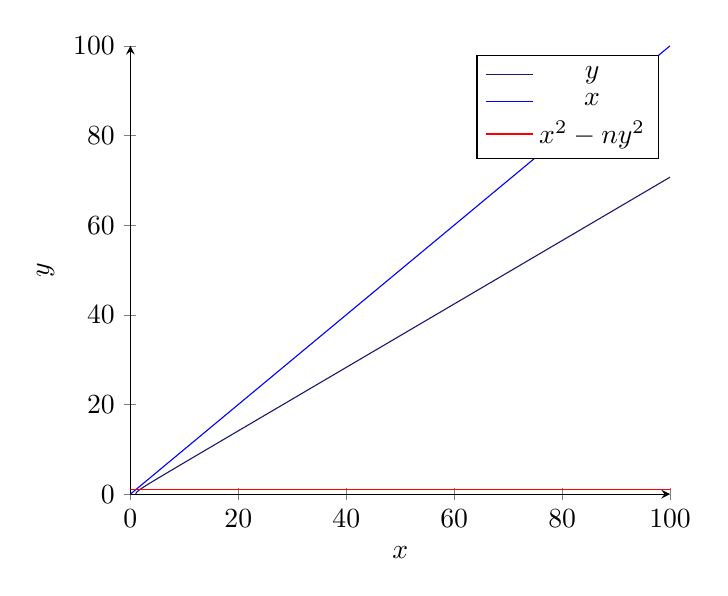
\begin{tikzpicture}
\begin{axis}[
    axis lines = left,
    xlabel = $x$,
    ylabel = {$y$},
]
\addplot [
    domain=0:100, 
    samples=1000, 
    color=MidnightBlue,
]
{((x^2 - 1)/2)^0.5};
\addlegendentry{$y$}
\addplot [
    domain=0:100, 
    samples=1000, 
    color=blue,
]
{x};
\addlegendentry{$x$}
\addplot [
    domain=0:100, 
    samples=1000, 
    color=red,
]
{1};
\addlegendentry{$x^2 - ny^2$}
\end{axis}
\end{tikzpicture}
\end{center}}
\end{mathbox}
%-----------------------------------------------------------------
\begin{phybox}{\text{\subsection{Toricelli's Theorm}}}
    {Torricelli’s theorem, also called Torricelli’s law, Torricelli’s principle, or Torricelli’s equation, statement that the speed, v, of a liquid flowing under the force of gravity out of an opening in a tank is proportional jointly to the square root of the vertical distance, $h$, between the liquid surface and the centre of the opening and to the square root of twice the acceleration caused by gravity, $2g$, or simply $v = \sqrt{2gh}$.
    
    The speed of a portion of water flowing through an opening in a tank a given distance, h, below the water surface is the same as the speed that would be attained by a drop of water falling freely under the force of gravity alone (that is, neglecting effects of air) through the same distance, h. The speed of efflux is independent of the direction of flow; at the point of the opening the speed is given by this equation, whether the opening is directed upward, downward, or horizontally.}
\end{phybox}
%----------------------------------------------------------------
\begin{chembox}{\text{\subsection{The Basic Principle of the Thermal World}}}
  {The first law of thermodynamics, also known as Law of Conservation of Energy, states that energy can neither be created nor destroyed; energy can only be transferred or changed from one form to another. For example, turning on a light would seem to produce energy; however, it is electrical energy that is converted.}
  \begin{align*}
  \Delta U = Q+W
  \end{align*}
  {Where $U$ is change in energy and $Q$ is heat added and $W$ is work done by system}
  {This law says that there are two kinds of processes, heat and work, that can lead to a change in the internal energy of a system. Since both heat and work can be measured and quantified, this is the same as saying that any change in the energy of a system must result in a corresponding change in the energy of the surroundings outside the system. In other words, energy cannot be created or destroyed. If heat flows into a system or the surroundings do work on it, the internal energy increases and the sign of q and w are positive. Conversely, heat flow out of the system or work done by the system (on the surroundings) will be at the expense of the internal energy, and q and w will therefore be negative.}
\end{chembox}
%---------------------------------------------------------------
\begin{mathbox}{\text{\subsection{Nooks and Corners}}}
{In mathematics, a parametric equation defines a group of quantities as functions of one or more independent variables called parameters. Parametric equations are commonly used to express the coordinates of the points that make up a geometric object such as a curve or surface (which are generally hard to express using linear equations and other such simpler ones), in which case the equations are collectively called a parametric representation or parameterization of the object.\\
Examples are parametric equations $a=\cos x$ and $b=\sin x$ are the parameterization of a unit circle with $x$ as the parameter such that $(a,b) = (\cos x, \sin x)$ are the co-ordinates.\\
\begin{center}
    \begin{tikzpicture}
    \draw[thick, dashed, red] (0,0) circle (1.5cm);
    \draw[thick, ->] (0,0) -> (-2,0);
    \draw[thick, ->] (0,0) -> (2,0);
    \draw[thick, ->] (0,0) -> (0,2);
    \draw[thick, ->] (0,0) -> (0,-2);
    \draw[thick, color=blue] (0,0) -- (1.0606,1.0606);
    \fill (1.0606,1.0606)  circle[radius=1.5pt, color=blue];
    \draw (1.0606,1.0606) node[right] {$(\cos x, \sin x)$};
    \draw[thick, color=red] (1.0606,0) -- (1.0606, 1.0606);
    \draw[thick, color=red] (0,0) -- (1.0606, 0);
    \draw (0.6, -0.2) node[south] {$\cos x$};
    \draw (1.06, 0.6) node[right] {$\sin x$};
    \end{tikzpicture}
\end{center}\\
\textbf{Explicit equations}\\
More generally, any curve given by an explicit equation
\begin{align*}
{\displaystyle y=f(x)}    
\end{align*}
\textbf{Parabola}\\
The simplest equation for a parabola is
\begin{align*}
    {\displaystyle y=x^{2}}
\end{align*}
\textbf{Circle}\\
Any circle can be parameterized by the following equation where $r$ is the radius of the circle.
\begin{align*}
{\displaystyle x^{2}+y^{2}=r^2}    
\end{align*}
\textbf{Ellipse}\\
An ellipse in canonical position (center at origin, major axis along the X-axis) with semi-axes a and b can be represented parametrically as
\begin{align*}
{\displaystyle {\begin{aligned}x&=a\,\cos t\\y&=b\,\sin t\end{aligned}}}    
\end{align*}
Parametric Equations are very useful in expressing geometric shapes using algebraic terms.}
\end{mathbox}
%---------------------------------------------------------------
\begin{phybox}{\text{\subsection{"Bulky" Modulus}}}
    {When we increase the pressure on a material by an amount $\Delta p$ ,it's density will increase.The fractional change in Volume will be $\frac{\Delta V}{V}$,which is negative if the volume decreases. The ratio between these quantities is called Bulk Modulus ($B$)
    \begin{align*}
        B = -\frac{P}{\Delta V / V}
    \end{align*}
    The Minus $(-)$ sign has been inserted in this definition to make $B$ positive,because $\Delta p$ and $v$ have opposite signs.}
\end{phybox}
%----------------------------------------------------------------
\begin{chembox}{\text{\subsection{Enthal/Ropy}}}
    \textbf{Enthalpy:}
   {When a process occurs at constant pressure, the heat evolved (either released or absorbed) is equal to the change in enthalpy.Enthalpy$(H)$ is the sum of the internal energy $(U)$ and Product of Pressure and Volume.}
    \begin{align*}
        H = U + PV
    \end{align*}\\
    Under constant Pressure
    \begin{align*}
        \Delta H = \Delta U + \Delta PV
    \end{align*}\\
    Under constant pressure and temperature\\
    \begin{align*}
        \Delta H = \Delta U + P \Delta V
    \end{align*}

    \textbf{Entropy:}
   {Entropy, the measure of a system’s thermal energy per unit temperature that is unavailable for doing useful work. Because work is obtained from ordered molecular motion, the amount of entropy is also a measure of the molecular disorder, or randomness, of a system. The concept of entropy provides deep insight into the direction of spontaneous change for many everyday phenomena. Its introduction by the German physicist Rudolf Clausius in 1850 is a highlight of 19th-century physics.}
   \begin{align*}
    S=k_b ln(\Omega)
   \end{align*}
   {Where $S$ is Entropy, $k_b$ is Boltzmann's constant and $\Omega$ is amount of microscopic observations.}
   \end{chembox}
%---------------------------------------------------------------
\begin{phybox}{\text{\subsection{Venturi's effect}}}
    {The Venturi effect is the reduction in fluid pressure that results when a fluid flows through a constricted section (or choke) of a pipe. The Venturi effect is named after its discoverer, Giovanni Battista Venturi.In fluid dynamics, an incompressible fluid's velocity must increase as it passes through a constriction in accord with the principle of mass continuity, while its static pressure must decrease in accord with the principle of conservation of mechanical energy (Bernoulli's principle). Thus, any gain in kinetic energy a fluid may attain by its increased velocity through a constriction is balanced by a drop in pressure.

    By measuring pressure, the flow rate can be determined, as in various flow measurement devices such as Venturi meters, Venturi nozzles and orifice plates.
    
    Referring to the adjacent diagram, using Bernoulli's equation in the special case of steady, incompressible, inviscid flows (such as the flow of water or other liquid, or low speed flow of gas) along a streamline, the theoretical pressure drop at the constriction is given by:}

    \begin{align*}
        p_1+p_2=\frac{\rho}{2} (v_2^2-v_1^2)  
    \end{align*}

    {where $\rho$, is the density of the fluid, $v_1$ is the (slower) fluid velocity where the pipe is wider, $v_2$ is the (faster) fluid velocity where the pipe is narrower }
     \\
    \textbf{Choked Flow}
    {The limiting case of the Venturi effect is when a fluid reaches the state of choked flow, where the fluid velocity approaches the local speed of sound. When a fluid system is in a state of choked flow, a further decrease in the downstream pressure environment will not lead to an increase in velocity, unless the fluid is compressed.

    The mass flow rate for a compressible fluid will increase with increased upstream pressure, which will increase the density of the fluid through the constriction (though the velocity will remain constant). This is the principle of operation of a de Laval nozzle. Increasing source temperature will also increase the local sonic velocity, thus allowing for increased mass flow rate but only if the nozzle area is also increased to compensate for the resulting decrease in density.}
    \\
    \textbf{Expansion of section}
    {The Bernoulli equation is invertible, and pressure should rise when a fluid slows down. Nevertheless, if there is an expansion of the tube section, turbulence will appear and the theorem will not hold. In all experimental Venturi tubes, the pressure in the entrance is compared to the pressure in the middle section; the output section is never compared with them.}
\end{phybox}
%---------------------------------------------------------------
\begin{phybox}{\text{\subsection{Heisenberg's Life Questioning Inequality}}}
{In quantum mechanics\footnote{Branch of Physics dedicated to observing the physical properties at the subatomic scale.}, the uncertainty principle (also known as Heisenberg's uncertainty principle) is a variety of mathematical inequalities asserting a fundamental limit to the accuracy with which the values for certain pairs of physical quantities of a particle, such as position ($x$) and momentum ($p$) can be predicted from initial or known conditions. Heisenberg, in simple words stated that if you know velocity/momentum of the particle, you can't find it's position and vice versa. The equation stated in favour;
\begin{align*}
    \Delta x \times \Delta P \geq \frac{h}{4\pi}
\end{align*}
where  $h = 6.626 \times 10^-34$ (Planck's Constant).\\
The more precisely the position of some particle is determined, the less precisely its momentum/velocity can be predicted from the known initial conditions.}
\end{phybox}
%------------------------------------------------------------
\begin{mathbox}{\text{\subsection{Catalan's Conjecture}}}
{The Catalan's conjecture, conjectured by the mathematician Eugène Charles Catalan in 1844 and proven in 2002 by Preda Mihăilescu. It states that there  exists only one solution to the equation
\begin{align*} 
    x^a - y^b = 1
\end{align*} 
where $x=3, a=2, y=2, b=3$ for {$a,b > 1$} and {$x,y > 0$}.}
\end{mathbox}
%---------------------------------------------------------------
\begin{phybox}{\text{\subsection{Magnus's effect}}}
    {The Magnus effect is an observable phenomenon that is commonly associated with a spinning object moving through air or another fluid. The path of the spinning object is deflected in a manner that is not present when the object is not spinning. The deflection can be explained by the difference in pressure of the fluid on opposite sides of the spinning object. The Magnus Effect depends on the speed of rotation.

    The most readily observable case of the Magnus effect is when a spinning sphere (or cylinder) curves away from the arc it would follow if it were not spinning. It is often used by football players, baseball pitchers and cricket bowlers. Consequently, the phenomenon is important in the study of the physics of many ball sports. It is also an important factor in the study of the effects of spinning on guided missiles—and has some engineering uses, for instance in the design of rotor ships and Flettner aeroplanes.
    
    Topspin in ball games is defined as spin about a horizontal axis perpendicular to the direction of travel that moves the top surface of the ball in the direction of travel. Under the Magnus effect, topspin produces a downward swerve of a moving ball, greater than would be produced by gravity alone. Backspin produces an upwards force that prolongs the flight of a moving ball}
\end{phybox}
%-----------------------------------------------------------------
\begin{chembox}{\text{\subsection{Entropy rules!}}}
    {The second law of thermodynamics says that the entropy of any isolated system always increases. Isolated systems spontaneously evolve towards thermal equilibrium—the state of maximum entropy of the system. More simply put: the entropy of the universe (the ultimate isolated system) only increases and never decreases.\footnote{RIP Universe. It is becoming more and more random with time.}

    A simple way to think of the second law of thermodynamics is that a room, if not cleaned and tidied, will invariably become more messy and disorderly with time – regardless of how careful one is to keep it clean. When the room is cleaned, its entropy decreases, but the effort to clean it has resulted in an increase in entropy outside the room that exceeds the entropy lost.}
\end{chembox}
%----------------------------------------------------------------
\begin{chembox}{\text{\subsection{Zero is weird}}}
    {The third law of thermodynamics states that the entropy of a system approaches a constant value as the temperature approaches absolute zero. The entropy of a system at absolute zero is typically zero, and in all cases is determined only by the number of different ground states it has. Specifically, the entropy of a pure crystalline substance (perfect order) at absolute zero temperature is zero. This statement holds true if the perfect crystal has only one state with minimum energy.}
\end{chembox}
%----------------------------------------------------------------
\begin{phybox}{\text{\subsection{Angular Momentum of an Electron}}}
{The {angular momentum} $(L)$ of an {electron} in the $n^{th}$ orbit is given by 
\begin{align*} 
    L = \frac{nh}{2\pi} 
\end{align*} where $h$ is the {Planck's constant}.}
\end{phybox}
%-------------------------------------------------------------------
\begin{chembox}{\text{\subsection{Gibbs Free Energy}}}
{In thermodynamics, the {Gibbs Free Energy} $(G)$ (named after Josiah Willard Gibbs) is a {thermodynamic potential} that calculates the {maximum reversible work} performed by a thermodynamic system at a {constant temperature} $(T)$ and pressure{} $(P)$. It is given by 
\begin{align*} 
    \Delta G=\Delta H-T\Delta S 
\end{align*} where $S$ represents its {Entropy}, i.e. the measure of randomness. {S.I unit - Joules}}
\end{chembox}
%-------------------------------------------------------------------
\begin{chembox}{\text{\subsection{Meme Time!}}}
    {In chemical thermodynamics, the fugacity of a real gas is an effective partial pressure which replaces the mechanical partial pressure in an accurate computation of the chemical equilibrium constant. It is equal to the pressure of an ideal gas which has the same temperature and molar Gibbs free energy as the real gas.}
    {Fugacities are determined experimentally or estimated from various models such as a Van der Waals gas that are closer to reality than an ideal gas. The real gas pressure and fugacity are related through the dimensionless fugacity coefficient. $\phi$}
    \begin{align*}
        \phi = \frac{f}{P}
    \end{align*}
    {Where $\phi$ is fugacity coeffiecient,$f$ is small pressure change and $P$ is large pressure change}
\end{chembox}
%-------------------------------------------------------------------
\begin{mathbox}{\text{\subsection{Inequalities}}}
    {In mathematics, an inequality is a relation which makes a non-equal comparison between two numbers or other mathematical expressions.
    It is used most often to compare two numbers on the number line by their size. There are several different notations used to represent different kinds of inequalities:
    \begin{itemize}
        \item{The notation $a < b$ means that $a$ is less than $b$.}
        \item{The notation $a > b$ means that $a$ is greater than $b$.}
    \end{itemize}
    In either case, a is not equal to b. These relations are known as strict inequalities, meaning that a is strictly less than or strictly greater than b. Equivalence is excluded.In contrast to strict inequalities, there are two types of inequality relations that are not strict:
    \begin{itemize}
        \item{The notation $a \leq b$  means that a is less than or equal to b (or, equivalently, at most b, or not greater than b).}
        \item{The notation $a \geq b$  means that a is greater than or equal to b (or, equivalently, at least b, or not less than b).}
    \end{itemize}
    There are many inequalities between means. For example, for any positive numbers $a_1, a_2, \dots a_n$ we have $H \leq G \leq A \leq Q$, where
    \begin{itemize}
        \item{$H = \frac{n}{\frac{1}{a_1} + \frac{1}{a_2} + \dots \frac{1}{a_n}}$}
        \item{$G = \sqrt[n]  {a_1 \cdot a_2 \cdot a_3 \cdot \dots a_n}$}
        \item{$A = \frac{a_1+a_2+a_3......a_n}{n}$}
        \item{$Q = \sqrt \frac{a_1^2 + a_2^2+a_3^2 \dots a_n^2}{n}$}
    \end{itemize}\\
    \textbf{A Problem:}\\
    Prove $a^2 + b^2 \geq 2ab$ for all integers $a, b$.\footnote{This is actually the first step/example in the road to prove $G \leq A.$}}
\end{mathbox}
%-------------------------------------------------------------------
\begin{phybox}{\text{\subsection{Half Life of Atoms}}}
    {Half-life represented by $t_\frac{1}{2}$ is the time required for a quantity to reduce to half of its initial value. It’s used in nuclear physics to describe how quickly unstable atoms undergo radioactive decay or how long stable atoms survive. Half-life is mainly defined in terms of probability; i.e. ”Half-life is the time required for exactly half of the entities to decay on average”. In other words, the probability of a radioactive atom decaying within its half-life is 50%.\\
    Exponential decay can be described by any of the following three equivalent formulas:
    \begin{align*}
    N(t)=N_{0}\left({\frac{1}{2}}\right)^{\frac{t}{t_{1/2}}}\\
    N(t)=N_{0}e^{-{\frac {t}{\tau }}}\\
    N(t)=N_{0}e^{-\lambda t}
    \end{align*}
    where;
    \begin{itemize}
    \item{$N_0$ is the initial quantity of the substance that will decay,}
    \item{$N(t)$ is the quantity that still remains and has not yet decayed after a time $t$,}
    \item{$t_\frac{1}{2}$ is the half-life of the decaying quantity, $\tau$ is a positive number called the mean lifetime of the decaying quantity,}
    \item{$\lambda$ is a positive number called the decay constant of the decaying quantity.}
    \end{itemize}
    The three parameters $t_\frac{1}{2}$, $\tau$, and $\lambda$ are all directly related in the following way:
    \begin{align*}
    t_\frac{1}{2}={\frac {\ln(2)}{\lambda }}=\tau \ln(2)
    \end{align*}}
    \end{phybox} 
%---------------------------------------------------------------------
